\subsection{Data}

In Section \ref{sec:inputdata} we mentioned that the real data used in this work needed to be manually cut out using a 50x50 window with just one object present in the image. Cropped images were then divided into 3 datasets: training, validation and testing dataset. Each dataset contains 50 images per class, giving a total of 300 images per dataset. However, to train the network, this is a very small amount of data. 
To increase the size of the dataset we implement augmentation techniques mentioned in the Section \ref{sec:parametersNetwork} and depicted in the Figure \ref{fig:agcutline}. This gives us a total of 1800 images for the training dataset used to fine-tune the network. 

\begin{figure}[!h]
   \centering
    \begin{subfigure}[t]{.15\textwidth}
        \centering
        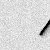
\includegraphics[width=\textwidth]{images/cutlineAg.png}
        \label{fig:cutlineag}
        \caption{}
    \end{subfigure}
    %\hfill
    \begin{subfigure}[t]{.15\textwidth}
        \centering
        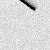
\includegraphics[width=\textwidth]{images/cutlineAg90.png}
        \label{fig:cutlineag90}
        \caption{}
    \end{subfigure}
    %\hfill
    \begin{subfigure}[t]{.15\textwidth}
        \centering
        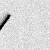
\includegraphics[width=\textwidth]{images/cutlineAg180.png}
        \label{fig:cutlineag180}
        \caption{}
    \end{subfigure}
    %\hfill
    \begin{subfigure}[t]{.15\textwidth}
        \centering
        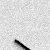
\includegraphics[width=\textwidth]{images/cutlineAg270.png}
        \label{fig:cutlineag270}
        \caption{}
    \end{subfigure}
    %\hfill
    \begin{subfigure}[t]{.15\textwidth}
        \centering
        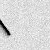
\includegraphics[width=\textwidth]{images/cutlineAgflipVodorovne.png}
        \label{fig:cutlineaghor}
        \caption{}
    \end{subfigure}
    %\hfill
    \begin{subfigure}[t]{.15\textwidth}
        \centering
        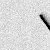
\includegraphics[width=\textwidth]{images/cutlineAgZvisle.png}
        \label{fig:cutlineagvert}
        \caption{}
    \end{subfigure}
    %\hfill
    \caption[Augmentation techniques applied to image of cut streak.]
    {Augmentation techniques applied to image of cut streak.(a) Original image, (b) Rotated by 90 °, (c) Rotated by 180 °, (d) Rotated by 270 °, (e) Flipped horizontally, (f) Flipped vertically. }
    \label{fig:agcutline}
\end{figure}
